\chapter{Fundamentals}
\label{sec:chapter2}
After introducing and motivating the problems this thesis focuses on in the previous chapter, this chapter gives an overview over the fundamentals of Human Action Recognition, Pose estimation as well as Neural Networks in general.

First, the fundamental concepts of Human Action recognition are discussed in Section \ref{sec:fund_har}, specifically in the context of video data.
Afterwards, $2D$ pose estimation for still images is introduced in Section \ref{sec:fund_poseestimation}.
Since many methods discussed in this thesis, including the approach by \cite{luvizon_2d/3d_2018}, use Neural networks, this thesis also introduces them in Section \ref{sec:neural_networks}, beginning with \textit{Artificial Neural networks} and how they are trained.
Afterwards, the use of \textit{Convolutional Neural networks}, often used in image processing, is motivated and explained.

\section{Human Action Recognition}
\label{sec:fund_har}
In \textit{Human Action Recognition}, often referred to simply by its acronym \textit{HAR}, the task is to attach a label of an \textit{action} to a signal, e.g. an image, video or sensor meassurements.
Thus, HAR is a \textit{classification} problem where the classes are human actions.
It is important to understand that HAR recognizes the action after it is completed, as opposed to \textit{action prediction}, which tries to predict the action while it is still happening \cite{kong_human_2018}.

Typical use-cases of Human Action Recognition consists of evaluating human behaviour, for example in a warehouse context \cite{reining_towards_2018}, or analyzing video surveillance footage \cite{htike_human_2014}.
An example of simple actions performed by multiple subjects is provided in \fref{fig:simple-actions}.

\begin{figure}[htb!]
    \centering
    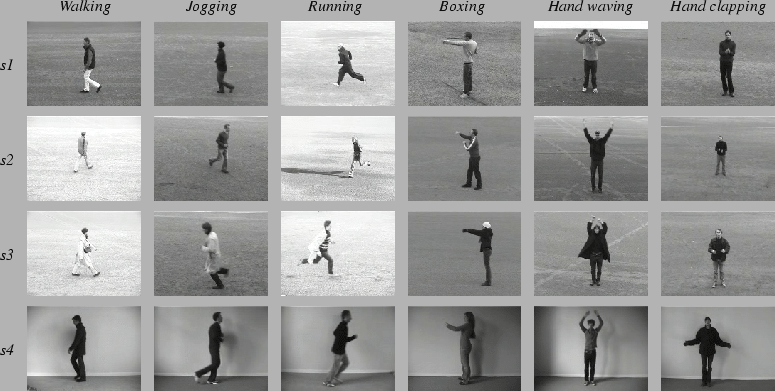
\includegraphics[width=0.8\textwidth]{simple-actions.png}
    \caption{Example of six actions performed by four different subjects, annotated with their corresponding label (top). Image taken from \cite{laptev_learning_2008}. }
    \label{fig:simple-actions}
\end{figure}

\subsection{Action Granularity}
When defining what an \textit{action} is, it is important to think about the degree of granularity needed.
As an illustration, consider an image of a person waving with her left hand at the camera.
It is not inherently clear whether the label attached to this action should be \textit{waving} or \textit{raising left arm}.
This is why the choice of labels is often domain and use-case specific.

According to \cite{zhang_review_2017}, human actions can be categorized into three levels, referred to as \textit{action primitives, activities and interactions}.
\textit{Action primitives} consists of actions where one part of the body is performing the actions.
For example, \textit{waving} or \textit{clapping} would constitute action primitives since a specific part of the body is responsible.
In contrast, \textit{activities} are actions where the whole body is involved in performing the action.
As an example, consider \textit{jumping} or \textit{jogging}.
When considering actions performed involving objects or other persons, e.g. \textit{shaking hands} or \textit{throwing a ball}, \cite{zhang_review_2017} categorize these actions as \textit{interactions}.

\subsection{Video-based HAR}
\label{sec:video-based-har}
When considering HAR on video clips, some domain-specific problems arise, which are outlined in \cite{zhang_review_2017}.

Firstly, depending on the camera and scene, the background of the image can be highly dynamic.
This means that the amount of information irrelevant for identifying the action can be very high and might change constantly.
As an example, consider a video filmed with a hand-held modern smart phone.
The camera is not stationary, so the background will shift while recording.
Also, depending on the scene, illumination changes and occlusion of the human subject might occur.

Secondly, different actions can have similar visual shapes.
Consider \textit{talking on the phone} and \textit{military salute}.
In both cases, the dominant hand is positioned at the side of the subjects head.
Depending on factors like image quality and the subjects rotation towards the camera, these two actions might be hard to differentiate.
Also, consider \textit{walking} and \textit{running}.
It is not inherently clear where the boundary between these two classes are, i.e., up to which point is a subject still \textit{walking} and when does the subject begin to \textit{run}?
This problem is referred to as \textit{interclass similarity}.
Another similar problem is the \textit{intraclass variation}, where the same action performed by different subjects might look very different.
As an example, consider \textit{throwing a ball}.
The scene will differ a lot when considering different clothing of the subject, different shape and color of the ball as well as different contexts where the action is happening, e.g., in a backyard or in a baseball stadium.
Also, performing actions at different intensities can alter their appearence, for example \textit{running} can be performed at slow to high speed and might even involve small jumps \cite{kong_human_2018}.

Thirdly, \cite{zhang_review_2017} mention \textit{group activities}.
When there are multiple subjects performing actions in a frame, it can be difficult to differentiate between many individual actions and a group action.
An example would be the difference between \textit{running} and \textit{playing football}.
Not only is a lot of context necessary to be able to determine a group activity but also to determine which subjects are part of the group activity and which are not.
Consider the case where, in a single frame, two subjects are playing football and two subjects are sitting, reading a book.
No single label is able to fully describe the human actions present in the image.
Thus, a sizeable portion of literature focuses on single human, single action problems.

\section{Pose Estimation}
\label{sec:fund_poseestimation}
\begin{figure}[htb!]
    \centering
    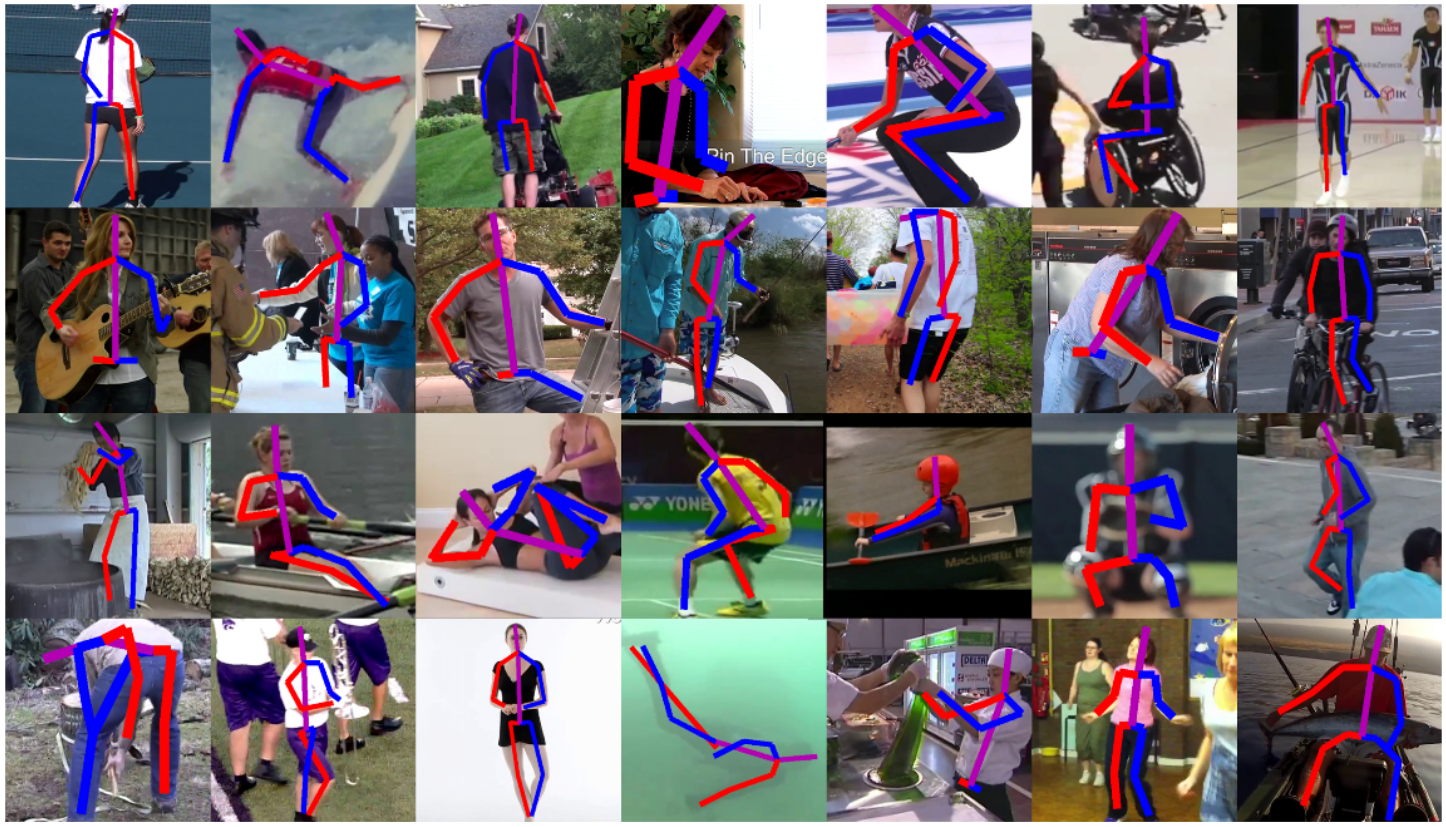
\includegraphics[width=0.9\textwidth]{tree-pose.png}
    \caption{Examples of human pose estimation. The pose is represented using a tree structure of joint positions, forming a skeleton. Image taken from \cite{newell_stacked_2016}.}
    \label{fig:tree-skeleton}
\end{figure}

Pose estimation is defined by modeling human joint positions from an image or from other signals.
In this thesis, however, the main focus is performing pose estimation using image-based methods, where the pixel positions for each joint are estimated.
The joint positions are then often represented in a tree structure representing a skeleton.
See \fref{fig:tree-skeleton} for an example.

Such a representation of the human pose is useful in many use-cases.
Action recognition on images, presented in Chapter \ref{sec:video-based-har}, often incorporates the pose of a human to identify the action performed by that human.
Additionally, since computer generated characters in movies become even more prevalent in recent years, pose estimation is often used for motion capturing, where an actor's pose is used for animating a computer generated character.

\begin{figure}[htb!]
    \centering
    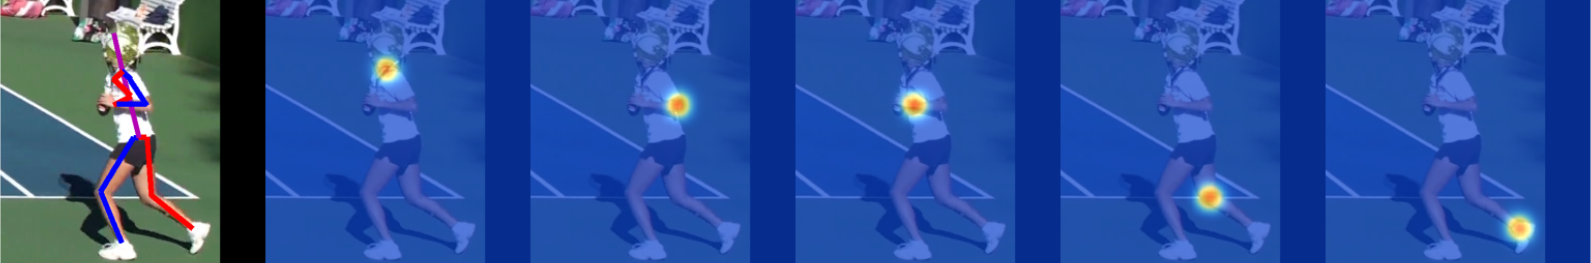
\includegraphics[width=0.9\textwidth]{2dheatmaps.png}
    \caption{Representing joint coordinates as probability heatmaps. From left to right: Tree structure representation of all joints, left shoulder, left elbow, left hand, right knee and right ankle. Image taken from \cite{newell_stacked_2016}.}
    \label{fig:probability-heatmaps}
\end{figure}

The skeleton structure shown is just a visualization of the data generated.
When computing pose, two main approaches are used.
Firstly, many approaches use regression to directly compute the image coordinates.
This approach was used in the early work because its reasoning is intuitive.
Secondly, heatmaps are used that represent a discrete probability distribution over the $x$ and $y$ coordinates.
One $2D$ heatmap corresponds to the position of one joint.
An example is provided in \fref{fig:probability-heatmaps}.
To extract the joint coordinates from heatmaps, a post processing step like the \textit{argmax} is needed.
According to \cite{luvizon_2d/3d_2018}, in practice, heatmap based methods outperform regression methods.

When computing pose from images, one obvious challenge is the variety in appearance because of different choices in \textbf{clothing}.
Consider the difference between detecting elbows in a picture with a person wearing a T-shirt and a picture with a person wearing a jacket.
Not only is the naked elbow exposed in the first example but the overall shape of the person is distorted because of the thick fabric of the jacket in the second example.
This problem also applies when considering the substantial differences in human appearance based on height and weight.

Other challenge are \textbf{occlusion} and \textbf{self-occlusion}. Occlusion happens when an object is in the line of sight of the camera, occluding parts of a joint or the whole joint.
Self-occlusion means that the subject in the image is positioned to the camera in such a way that their own body occludes the joints.

When focusing on detecting the pose of a single human, other \textbf{humans in the background} might complicate the process because their joints could be wrongly recognized as belonging to the desired subject.
Consider again the examples provided in \fref{fig:tree-skeleton}.
It is easy to see how such errors can occur in crowded environments.

According to \cite{zhu_articulated_2016}, there are two general approaches for pose estimation.
First, in \textit{top-down pose estimation}, a generic model of a human is used as a starting point.
This model is then updated based on the information gathered from the images.
That way, there is always a model where all joints are present, i.e., occlusion is handled easily.
This approach, however, requires a priori assumptions about the human body and may lead to bad results when these assumptions are not true, i.e., people with disabilities or exceptionally tall or heavy people.
Second, \textit{bottom-up pose estimation} focuses on detecting individual body parts.
These individual parts can then be combined together into the final pose representation.
As part detectors got significantly more accurate in recent years due to the development of \textit{deep convolutional neural networks}, this is the predominant approach for pose estimation in the current literature.


\section{Neural Networks}
\label{sec:neural_networks}
Neural networks are becoming increasingly popular in modern computer vision and machine learning pipelines due to their high classification accuracy.
In the following chapter, an introduction into their functionality is given, starting with the McCulloch-Pitts-Neuron.
Then, the Perceptron is discussed, which generalizes the McCulloch-Pitts-Neuron to real numbers.
Also, an outline of how Perceptrons learn from data is presented.
Afterwards, multiple Perceptrons are combined into a network to solve more complex tasks.
Finally, convolutional neural networks are discussed, which are very commonly used in modern computer vision literature due to their ability to learn how to extract meaningful visual features from data.

\subsection{Artificial Neural Networks}
Artificial Neural Networks are unidirected graphs where \textit{neurons} are used as vertices.
A neuron is a compute unit, which performs an action upon its inputs and propagates its output along the output edge.
Each neuron has a set of internal parameters that determine how its output is computed.
In the following sections, two approaches for how a neuron is defined are presented, as well as mechanisms for determining their internal parameters automatically.
Also, the approach of constructing a neural network from a collection of neurons to compute more complex functions will be discussed.

\subsubsection{McCulloch-Pitts-Neuron}
\label{sec:mcculloch-pitts}
One of the earliest definitions of a neuron was proposed by Warren McCulloch and Walter Pitts in 1943 \cite{mcculloch_logical_1943}.
The McCulloch-Pitts-Neuron (MCP), also referred to as the McCulloch-Pitts unit, takes binary input values $\bm{x} = (x_1, \dots, x_n) \in \mathbb{B}^n$ and computes a binary value $f(\bm{x}) \in \mathbb{B}^n$.
Additionally, the neuron contains a threshold value $\theta \in \mathbb{N}$.
After adding all input signals, the sum (also referred to as \textit{excitation}) is compared to $\theta$ \eref{eq:mcculloch-binary}.
The output of the neuron is $1$ if the excitation is greater or equal to $\theta$ and $0$ otherwise.

\begin{equation}
    \begin{split}
        \label{eq:mcculloch-binary}
        f(\bm{x}, \theta)
        &=
        \begin{cases}
            1 & \text{if } \sum_{i=0}^n x_i \geq \theta \\
            0 & \text{otherwise}
        \end{cases}
%        \\
%        &= \phi(\psi(\bm{x}), \theta)
    \end{split}
\end{equation}

This simple neuron is capable of realizing some binary operators by choosing different values for $\theta$.
For example, the \textbf{boolean OR} operator is realized by setting $\theta = 1$ and the \textbf{boolean AND} operator (over $n$ inputs) can be implemented by choosing $\theta = n$ \cite{rojas_neural_1996}.

A geometrical explanation of how the MCP works is that it separates its input space into two half-spaces, assigning the output $1$ to all input combinations on one side and $0$ on the other.
For example, for two dimensional input spaces (two input variables $x_1$ and $x_2$), a MCP defines a separating line while for three dimensional input spaces the MCP becomes a separating hyperplane.
A visualization for the \textbf{boolean OR} function with three input variables is shown in \fref{fig:mcp-geometric-or}.

\begin{figure}[htb!]
    \centering
    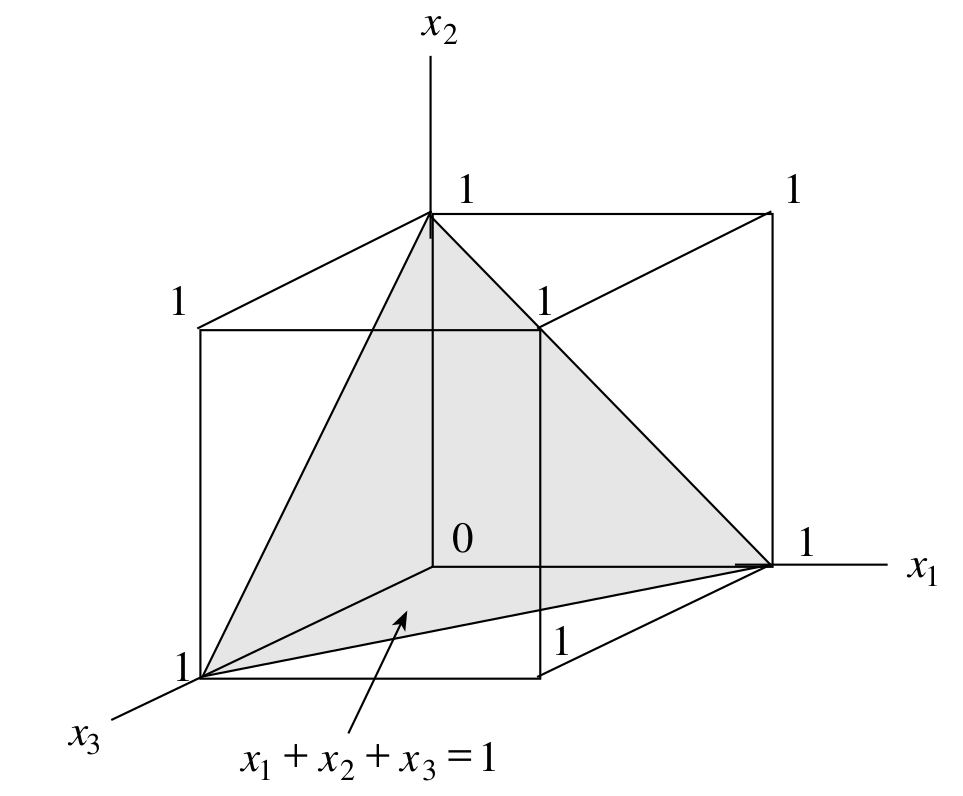
\includegraphics[width=0.6\textwidth]{mcp-geometric-or.png}
    \caption{Example of MCP dividing the three-dimensional input space using a hyperplane. The MCP is configured to model the \textbf{boolean OR} function. Image taken from \cite{rojas_neural_1996}.}
    \label{fig:mcp-geometric-or}
\end{figure}

The MCP looked at so far is also called an \textit{uninhibited} MCP.
\cite{rojas_neural_1996} show that \textit{uninhibited} MCP's can only model monotonic logical functions.
By adding \textit{inhibitory inputs} $\bm{y} = (y_1, \dots, y_m) \in \mathbb{B}^m$ to the MCP, however, non-monotonic logical functions like \textbf{boolean NOT} can be implemented.
The output of the MCP changes to

\begin{equation}
    \hat{f}(\bm{x}, \bm{y}, \theta) = f(\bm{x}, \theta) \cdot \prod_{j = 0}^m (1 - y_j).
\end{equation}

With \textit{uninhibited} and \textit{inhibited} inputs a neuron can model any conjugation of negated and non-negated inputs.
For example, modeling the boolean function $x_1 \wedge \neg x_2 \wedge x_3$ results to

\begin{equation}
    \label{eq:conjunction-negated}
    \hat{f}(x_1, x_2, x_3, \theta=1) = f(x_1, x_3, \theta) \cdot (1 - x_2).
\end{equation}

\begin{figure}[htb!]
    \centering
    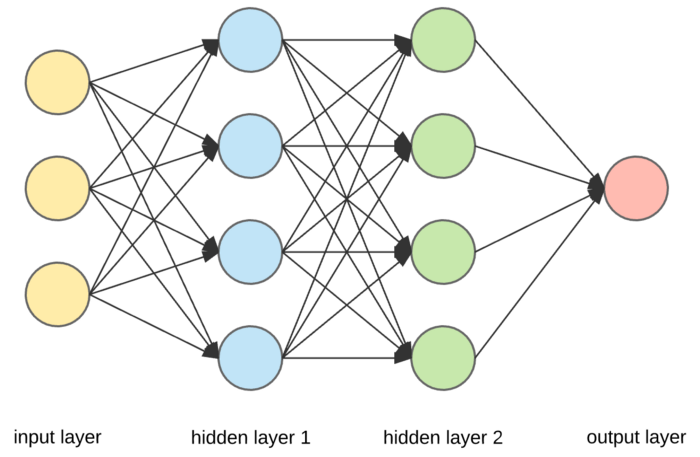
\includegraphics[width=0.6\textwidth]{simple-neural-network.png}
    \caption{Example of a simple neural network, made up of two hidden layers. Image taken from \cite{dertat_applied_2017-1}.}
    \label{fig:simple-neural-network}
\end{figure}

To compute more complex functions, multiple neurons can be grouped together into \textit{layers}, which, in turn, are connected into a \textit{neural network}.
An example of a neural network made up from multiple layers can be seen in \fref{fig:simple-neural-network}.
The input layer does not contain neurons, however, since the nodes to not perform any computation.
Rather, the input layer abstracts the input values into the neural network framework.
Any layer between the input layer and the final layer is referred to as an \textit{hidden layer}.
Each neuron in a layer receives the output of all neurons in the previous layer as input.
When defining the number of layers a network has, the input layer is typically not counted because it does not contain compute units.
This means that the example network in \fref{fig:simple-neural-network} would be considered a three layer network.

By using a two-layer neural network it is possible to model any boolean function $f: \mathbb{B}^n \to \mathbb{B}$.
The first layer consists of neurons that model conjunctions over the inputs just as presented above.
The second layer is made up of a single neuron, which is configured to compute \textbf{boolean OR}.
By making the outpus of the first layer the input of the disjunction in the second layer any boolean function $f$ can be computed because any such function can be represented in disjunctive normal form.

The obvious limitation of McCulloch-Pitts-Networks is that they are limited to the domain of logical functions.
Additionally, they have to be constructed rather than being able to learn the desired function because they rely on fixed connections to model relations between input variables.

\subsubsection{Perceptron}

In contrast to the McCulloch-Pitts-Neuron, a Perceptron uses real valued inputs $\bm{x} = (x_1, \dots, x_n) \in \mathbb{R}^n$ as well as a set of real valued weights $\bm{w} = (w_1, \dots, w_n) \in \mathbb{R}^n$:

\begin{equation}
    f(\bm{x}, \bm{w}, \theta) =
    \begin{cases}
        1 & \text{if } \sum_{i=0}^n w_i \cdot x_i \geq \theta \\
        0 & \text{otherwise.}
    \end{cases}
\end{equation}

Instead of setting $\theta$ as part of the neuron it is preferred to treat it as an additional trainable parameter.
To achieve this, a new fixed input value $x_b = 1$ with the corresponding weight $w_b = -\theta$ is added to the model and the previously \emph{internal} $\theta$ is fixed to $0$ \eref{eq:full-perceptron}.
This additional weight is called the \textit{bias} of the Perceptron.

\begin{equation}
    \label{eq:full-perceptron}
    f(\bm{x}, \bm{w}) =
    \begin{cases}
        1 & \text{if } ~ -w_b + \sum_{i=0}^n w_i \cdot x_i \geq 0 \\
        0 & \text{otherwise}
    \end{cases}
\end{equation}

For notational convenience, from now on the bias is assumed to be part of $\bm{w}$, i.e., $\bm{w} = (w_1, \dots, w_n, -\theta)$ and the additional input $x_b = 1$ is part of $\bm{x}$, i.e., $\bm{x} = (x_1, \dots, x_n, 1)$.

The \textit{excitation} of a Perceptron is still just a (weighted) linear combination.
This means that the Perceptron, like the MCP, separates the input space by a hyperplane.
In \fref{fig:perceptron-logic} examples for some common logical functions for two input variables are provided.

\begin{figure}[htb!]
    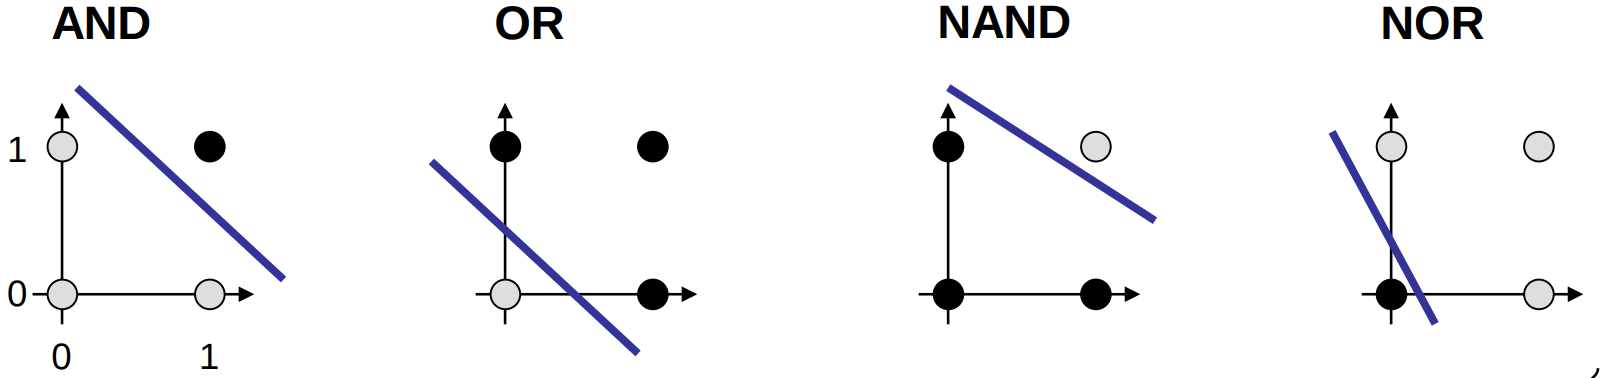
\includegraphics[width=0.9\textwidth]{perceptron-linear-seperable.png}
    \caption{Logical functions modelled by a single Perceptron. The blue line indicates where the input space is divided. All input combinations on one side of the line are going to be assigned to $1$ while being assigned to $0$ on the other side. Notice that there are infinitely many possibilities for dividing lines since the input space is real valued. Image taken from \cite{rudolph_lecture_2018}.}
    \label{fig:perceptron-logic}
\end{figure}

While MCP's were designed to model logical functions like \textbf{boolean OR} or \textbf{boolean AND} by setting $\theta$ as well as categorizing the input variables as either \textit{inhibitory} or \textit{non-inhibitory}, Perceptrons are able to infer these parameters through a \textit{learning process}.

Perceptrons learn from a \textit{training set} $\bm{M} = \bm{P} \cup \bm{N}$ comprised of \textit{positive examples} and \textit{negative examples}.
A positive example $\bm{p} \in \bm{P}$ is defined as an input for which the Perceptron should output $1$.
Analogously, the Perceptron should output $0$ for each negative example.
Learning in the context of Perceptrons then means determining a parameter vector $\bm{w}$, which satisfies the following inequalities for all positive and negative examples:

\begin{equation}
    \begin{split}
        \bm{w} \cdot \bm{p} &\geq 0 ~ \forall \bm{p} \in \bm{P} \\
        \bm{w} \cdot \bm{n} &< 0 ~ \forall \bm{n} \in \bm{N}.
    \end{split}
\end{equation}

A parameter vector, which satisfies these inequalities, then defines the hyperplane separating positive from negative training examples.
The Perceptron can then assign an output value to non-training examples by computing its output using the learned weight vector.
The training examples are required to be linearly separable in order to find an optimal separating hyperplane.

The general algorithmic approach determining an optimal weight vector is the following:

\begin{enumerate}
    \item Start with a random weight vector $\bm{w}$
    \item Evaluate how accurate the hyperplane defined by $\bm{w}$ separates the input space
    \item If all positive and negative examples are separated correctly:
    \begin{enumerate}
        \item \textbf{Done}
    \end{enumerate}
    \item Else
    \begin{enumerate}
        \item Update weight vector in a way which further reduces the error function
        \item Go to step 2
    \end{enumerate}
\end{enumerate}

For the learning algorithm to determine the accuracy of a given weight vector $\bm{w}_i$, an \textbf{error function} or \textbf{loss function} needs to be provided.
Such a function takes all positive and negative examples and calculates the amount of error, i.e., number of wrongfully classified examples.

One example of a loss function is the \textbf{sum of squared error} function:

\begin{equation}
    \label{eq:sse-loss}
    SSE(\bm{w}) = \sum_{\bm{x} \in \bm{M}} (\hat{f}(\bm{x}, \bm{w}) - y_x)^2.
\end{equation}

This function computes the output of the Perceptron $\hat{f}(\bm{x}, \bm{w})$ for a given weight vector $\bm{w}$ and subtracts the expected output $y_x$ for the input $\bm{x}$.
It is trivial to see that the minimum error $SSE(\bm{w}) = 0$ is achieved if and only if $\hat{f}(\bm{x}) = 1$ for all positive examples and $\hat{f}(\bm{x}) = 0$ else.

Iteratively updating the weight vector needs a strategy that guarantees that the error will be less than it was before after updating.
One algorithm, presented in \cite{rojas_neural_1996} and simply called \textit{Perceptron learning algorithm}, uses the following method.

\begin{figure}[htb!]
    \centering
    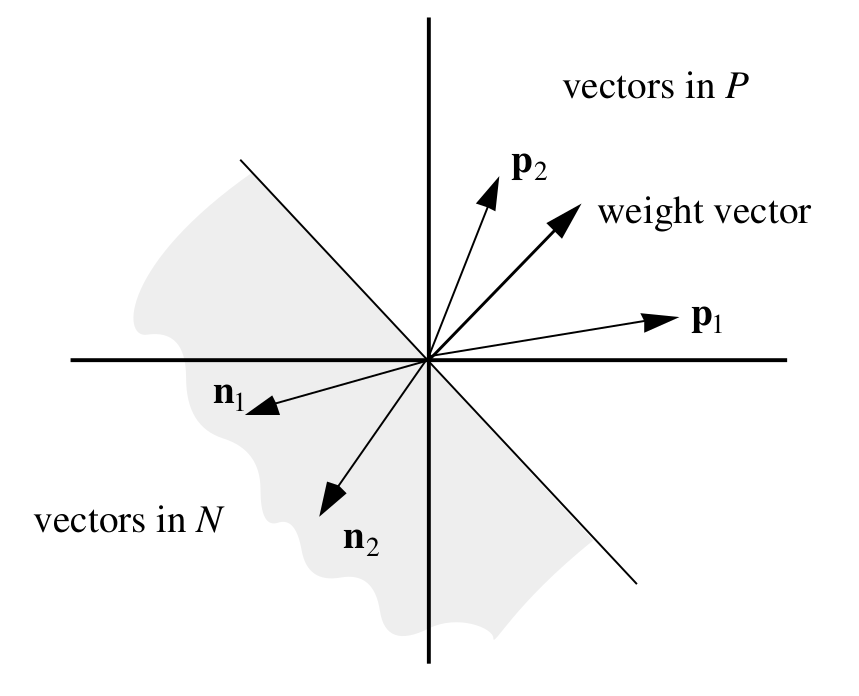
\includegraphics[width=0.55\textwidth]{perceptron-learning-update.png}
    \caption{Visualization of the weight plane $\bm{w} \cdot \bm{x}$ separating two positive and two negative vectors. The weight vector $\bm{w}$ is the normal of the hyperplane. Image taken from \cite{rojas_neural_1996}}
    \label{fig:perceptron-learning-update}
\end{figure}

A training example $x \in M$ is chosen randomly.
Also, as discussed before, a random weight vector $\bm{w}_t = \bm{w}_0$ is initialized.
If $x \in P$ and $\bm{w}_t \cdot x \leq 0$ then the weight vector needs to be updated.
The idea is that, in the case above, the two vectors $\bm{x}$ and $\bm{w}$ must have an angle bigger than 90 degrees (see \fref{fig:perceptron-learning-update}).
By rotating $\bm{w}$ towards $\bm{x}$ the angle will be reduced, eventually putting $\bm{x}$ on the correct side of the hyperplane.
To rotate $\bm{w}$ the algorithm proposes $\bm{w}_{t+1} = \bm{w}_{t} + \bm{x}$.
Analogously, if $x \in N$ and $\bm{w}_t \cdot x \geq 0$ the algorithm proposes $\bm{w}_{t+1} = \bm{w}_{t} - \bm{x}$.
This is done for each $x \in M$ in a random order.

As $P$ and $N$ are required to be linearly separable and there are a finite number of examples it can be proven that, after a finite amount of steps, the error will be reduced to zero and the hyperplane will correctly separate the two sets \cite{rojas_neural_1996}.

\subsubsection{Gradient Descent Learning}
\label{sec:gradient_descent}
Another approach to learning the weights of a Perceptron is \textit{gradient descent}.
Given an error function $E$ with a set of initial weights $\bm{w_t}$ and an input example $\bm{x}$ the amount of error is given by $E(\bm{w}, \bm{x})$.
If the error function is differentiable, one can calculate the gradient of the error function for each weight $w_i \in \bm{w}$ using

\begin{equation}
    \frac{\partial E}{\partial w_i},
\end{equation}

which points toward the steepest ascend of the error function.

Consider the error function defined earlier in \eref{eq:sse-loss}.
The partial derivative given each $w_i \in \bm{w}$ is then given by:

\begin{equation}
    \label{eq:error-derivative-1}
    \begin{split}
        \frac{\partial SSE(\bm{M}, \bm{w})}{\partial w_i}
        &= \frac{\partial }{\partial w_i} \left( \sum_{x \in \bm{M}} (\hat{f}(\bm{x},\bm{w}) - y_x)^2 \right) \\
        &= \sum_{x \in \bm{M}} \frac{\partial }{\partial w_i} (\hat{f}(\bm{x},\bm{w}) - y_x)^2 \\
        &= 2 \cdot \sum_{x \in \bm{M}} \hat{f}(\bm{x},\bm{w}) - y_x) \cdot  \frac{\partial }{\partial w_i} (\hat{f}(\bm{x}, \bm{w}) - y_x) \\
        &= 2 \cdot \sum_{x \in \bm{M}} \hat{f}(\bm{x},\bm{w}) - y_x) \cdot  \frac{\partial }{\partial w_i} \hat{f}(\bm{x}, \bm{w}).
    \end{split}
\end{equation}

This presents a challenge, however, since $\hat{f}(\bm{x}, \bm{w})$ is not differentiable.
Until now, the definition of a single Perceptron was the following:

\begin{equation}
    \begin{split}
        \hat{f}(\bm{x}, \bm{w})
        &=
            \begin{cases}
                1 & \text{if } \bm{w} \cdot \bm{x} \geq 0 \\
                0 & \text{otherwise}
            \end{cases}
        \\
        &= \phi(\bm{x} \cdot \bm{w})
        \\
        &= \phi(\psi(\bm{x}, \bm{w})),
    \end{split}
\end{equation}

where $\psi$ is called the \textit{integration function}, which computes the excitation and $\phi$ the \textit{activation function} that computes the activation of the neuron.

This results in a non-differentiable activation function since the thresholding approach is not continuous, which means that it cannot be differentiable.
A popular choice for a differentiable activation function is the \textit{sigmoid activation function} $S(x)$ given by:

\begin{equation}
    S(x) = \frac{1}{1 + e^{-x}}.
\end{equation}

One can easily see that the sigmoid function is differentiable and that the derivative is given by:

\begin{equation}
    \begin{split}
        \frac{d}{dx} S(x)
        &= \frac{e^{-x}}{(1 + e^{-x})^2} \\
        &= S(x)(1 - S(x)).
    \end{split}
\end{equation}

By then choosing $\phi = S$ and keeping $\psi(\bm{x}, \bm{w}) = \bm{x} \cdot \bm{w}$ in \eref{eq:error-derivative-1} the partial derivative of the error function becomes:

\begin{equation}
    \label{eq:error-derivative-2}
    \begin{split}
        \frac{\partial SSE(\bm{M}, \bm{w})}{\partial w_i}
        &= 2 \cdot \sum_{x \in \bm{M}} (\hat{f}(\bm{x},\bm{w}) - y_x) \cdot  \frac{\partial }{\partial w_i} \hat{f}(\bm{x}, \bm{w}) \\
        &= 2 \cdot \sum_{x \in \bm{M}} (S(\bm{x} \cdot \bm{w}) - y_x) \cdot  \frac{\partial }{\partial w_i} S(\bm{x} \cdot \bm{w}) \\
        &= 2 \cdot \sum_{x \in \bm{M}} (S(\bm{x} \cdot \bm{w}) - y_x) \cdot  \frac{\partial }{\partial w_i} S \left(\sum_j x_j \cdot w_j \right) \\
        &= 2 \cdot \sum_{x \in \bm{M}} (S(\bm{x} \cdot \bm{w}) - y_x) \cdot  S(\bm{x} \cdot \bm{w}) \cdot (1-S(\bm{x} \cdot \bm{w})) \cdot \frac{\partial }{\partial w_i} \sum_j x_j \cdot w_j \\
        &= 2 \cdot \sum_{x \in \bm{M}} (S(\bm{x} \cdot \bm{w}) - y_x) \cdot  S(\bm{x} \cdot \bm{w}) \cdot (1-S(\bm{x} \cdot \bm{w}))\cdot x_i.
    \end{split}
\end{equation}

After computing the partial derivative for each $w_i \in \bm{w}$ the \textit{gradient} then is given by:

\begin{equation}
    \nabla SSE(\bm{M}, \bm{w}) = \left(\frac{\partial SSE(\bm{M}, \bm{w})}{\partial w_1}, \dots, \frac{\partial SSE(\bm{M}, \bm{w})}{\partial w_n} \right).
\end{equation}

Finally, the current weights $\bm{w_t}$ can be updated by changing the weights by a certain \textit{step size or learning rate} $\gamma$ towards a local minimum of the error function by applying

\begin{equation}
    \label{eq:gradient-binary-update}
    \bm{w_{t+1}} = \bm{w_t} - \gamma ~ \nabla SSE(\bm{M}, \bm{w}).
\end{equation}

Since the gradient points toward the steepest ascent of the error function a negation is needed to approach the local minimum.

\subsubsection{Multi-Layer Perceptron}
The assumption was made that the two sets of points $P$ and $N$ are linearly separable.
Many problems, however, are more complex and cannot be easily separated linearly.
One example from the realm of logical functions is the \textbf{XOR} function.
As an example, consider \textbf{XOR} with two input variables.
If visualized in the same way as in \fref{fig:perceptron-logic} it is quite trivial to see that no single line is able to divide the positive from the negative points.
A more complex model is necessary for modeling functions with \textit{convex solution spaces} such as \textbf{XOR} \fref{fig:xor-convex}.
Similar to \ref{sec:mcculloch-pitts}, Perceptrons can be arranged into layers to compute more complex functions.
Such a network is also known as a \textit{multi-layer perceptron (MLP)}.

\begin{figure}[htb!]
    \centering
    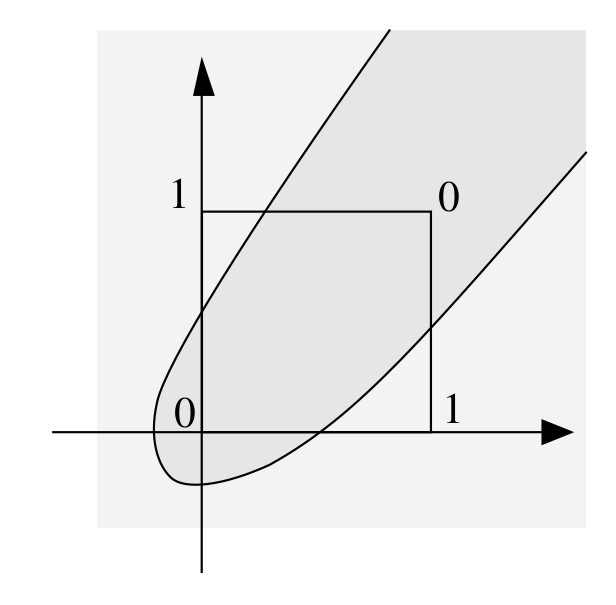
\includegraphics[width=0.5\textwidth]{xor-convex.png}
    \caption{Solving the \textbf{XOR} problem by using separating \textit{regions} instead of hyperplanes. Image taken from \cite{rojas_neural_1996}}
    \label{fig:xor-convex}
\end{figure}

By constructing an MLP with one input layer, one hidden layer as well as one output layer, the network is capable of modeling every convex solution space \cite{rojas_neural_1996}.
The Perceptrons in the hidden layer each learn to linearly separate the solution space into two parts like described earlier.
By using just one Perceptron in the second layer, which is able to learn the \textbf{boolean AND} function over all outputs from the previous layer it is possible to learn any convex solution space.
A visualization is provided in \fref{fig:convex-solution}.

\begin{figure}[htb!]
    \centering
    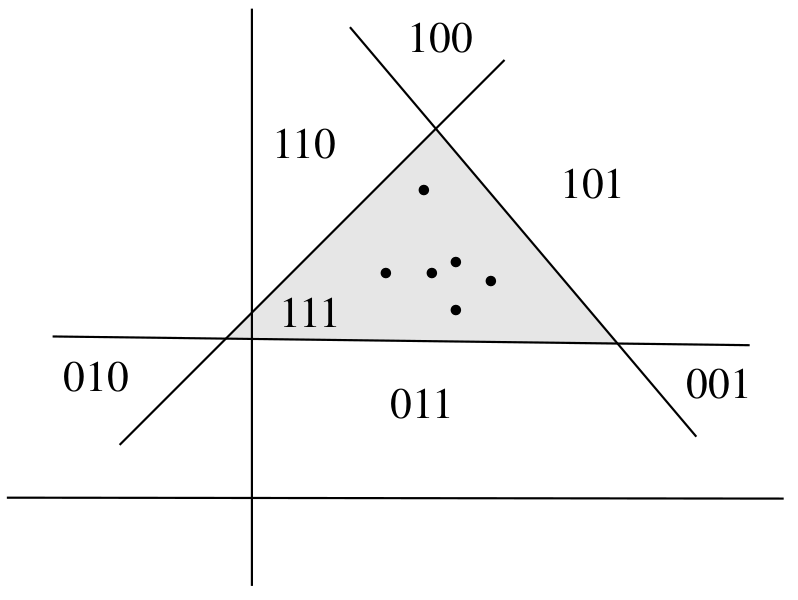
\includegraphics[width=0.8\textwidth]{convex_solution_space.png}
    \caption{Example of a convex solution space using a two-layered MLP with three Perceptrons in the first and one Perceptron in the second layer. Each bit vector $b = (x_1, x_2, _3)$ shows the output of Perceptron 1, 2 and 3 respectively. Image taken from \cite{rojas_neural_1996}}
    \label{fig:convex-solution}
\end{figure}

Even with the ability to model any convex solution space, there are still problems which have a \textit{non-convex solution space}.
However, by adding another hidden layer to the MLP these problems can also be solved.

The first hidden layer behaves just like in the previous example with each Perceptron splitting the input space into two.
Each Perceptron in the second layer again learns \textbf{boolean AND} functions, resulting in as many convex regions as there are neurons in the layer.
In the third layer, a Perceptron then combines these regions into non-convex regions using the learned \textbf{boolean OR} operator.
In fact, a three-layer MLP is able to model any arbitrary function (given enough Perceptrons per layer) \cite{rojas_neural_1996}.

\subsubsection{Backpropagation}
A single Perceptron can be trained using gradient descent.
A network of many Perceptrons, however, a different algorithm is needed.

Probably the most common learning algorithm for training MLPs is the \textbf{backpropagation algorithm}, initially proposed by \cite{werbos_beyond_1974} and popularized by \cite{rumelhart_learning_1986}.
It uses gradient descent with the addition of propagating the error backwards through the network by making use of the chain rule of derivation.

For each example $\bm{x_i}$ in the training data, the algorithm follows these steps:

\begin{enumerate}
    \item Start with random weights $\bm{W}_0 = (\bm{w_0}, \dots, \bm{w_n})$ for each neuron.
    \item Feed $\bm{x_i}$ into the network (called a \textit{forward pass})
    \begin{itemize}
        \item $\hat{f}(\bm{x_i}, \bm{w}_0) = \bm{y_i}$
    \end{itemize}
    \item Compute gradient at the last layer by using a loss function and the expected result $\hat{\bm{y_i}}$.
    \item Compute gradient for the previous layers, incorporating the error from the consecutive layers (called a \textit{backward pass}).
    \item Update the weights with their corresponding gradients.
\end{enumerate}

In order to show how the Backpropagation algorithm works consider a MLP with one hidden layer $L_1$, one output layer $O_1$ and $n$ inputs.
Also, let $\lVert L_1 \rVert = \lVert O_1 \rVert = M$ without loss of generality.

First, the forward pass is performed.
The output of each neuron $h_j(\bm{x}, \bm{w_j}) = y_j$ in the hidden layer can be described using the following equation:

\begin{equation}
    \begin{split}
        h_j(\bm{x}, \bm{w_j})
        &= S(\bm{x} \cdot \bm{w_j}) \\
        &= \frac{1}{1 + e^{-(\bm{x} \cdot \bm{w_j})}}.
    \end{split}
\end{equation}

Similarly, after the output layer, the output $g_k$ for each neuron given the network input can be described as:

\begin{equation}
    \begin{split}
        g_k(\bm{x}, \bm{w_k})
        &= S\left(\sum_{j=0}^M w_{jk} \cdot h_j(\bm{x}, \bm{w_j})\right) \\
        &= S\left(\sum_{j=0}^M w_{jk} \cdot S \left(\sum_{i=0}^N w_{ij} \cdot x_i\right)\right).
    \end{split}
\end{equation}

Every differentiable loss function can be used in the Backpropagation algorithm.
For consistency, consider the \textit{sum of squared error} function defined in \eref{eq:sse-loss}.
After the forward pass through the network the loss for a single output neuron $g_k$ is given by:

\begin{equation}
    \begin{split}
        SSE(\bm{x}, (\bm{w_j}, \bm{w_k}))
        &= (y_k - \hat{y}_{k})^2 \\
        &= (g_k(\bm{x},\bm{w_k}) - \hat{y}_{k})^2 \\
        &= \left(S \left(\sum_{j=0}^M w_{jk} \cdot h_j(\bm{x}, \bm{w_j})\right) - \hat{y}_{k}\right)^2 \\
        &=  \left( S\left(\sum_{j=0}^M w_{jk} \cdot S \left(\sum_{i=0}^N w_{ij} \cdot x_i\right)\right) - \hat{y}_{k}\right)^2
    \end{split}
\end{equation}

By using the same approach as with gradient descent, the partial derivative of the loss function with regards to the weights of the output layer is given by:

\begin{equation}
    \begin{split}
        \frac{\partial ~ SSE(\bm{x}, \bm{w})}{\partial w_{jk}}
        &= \frac{\partial}{\partial w_{jk}} (g_k(\bm{x},\bm{w_k}) - \hat{y}_{k})^2.
    \end{split}
\end{equation}

Using the chain rule for derivation

\begin{equation}
    (p(b(x)))' = p'(b(x)) \cdot b'(x),
\end{equation}

the partial derivative can be broken down :

\begin{equation}
    \label{eq:vanishing_1}
    \begin{split}
        \frac{\partial ~ SSE(\bm{x}, \bm{w})}{\partial w_{jk}}
        &= \frac{\partial}{\partial w_{jk}} ~ (g_k(\bm{x},\bm{w_k}) - \hat{y}_{k})^2 \\
        &= 2 \cdot (g_k(\bm{x},\bm{w_k}) - \hat{y}_{k}) \cdot  S'\left(\sum_{j=0}^M w_{jk} \cdot h_j(\bm{x}, \bm{w_j})\right) \cdot h_j(\bm{x}, \bm{w}_j) \\
        &= 2 \cdot (y_k - \hat{y}_{k}) \cdot  y_k \cdot (1 - y_k) \cdot h_j(\bm{x}, \bm{w_j}) \\
        &= \delta_k \cdot h_j(\bm{x}, \bm{w_j}) \\
        &= \delta_k \cdot y_j.
    \end{split}
\end{equation}

One can observe that the output of all neurons from layer $N_{k}$ are needed to compute the partial derivate for neurons in layer $N_{k+1}$, which is why the initial forward pass through is necessary.

Similarly, the partial derivative of the loss function with regards to $w_{ij}$ is given by \eref{eq:backprop-partial-hidden}.
However, while running Backpropagation, the partial derivatives of all nodes in layer $N_{k+1}$ need to be computed in order to determine the partial derivative of nodes in layer $N_{k}$ \cite{rojas_neural_1996}.

\begin{equation}
    \label{eq:backprop-partial-hidden}
    \begin{split}
        \frac{\partial ~ SSE(\bm{x}, \bm{w})}{\partial w_{ij}}
        &= \frac{\partial}{\partial w_{ij}} ~ (g_k(\bm{x},\bm{w_k}) - \hat{y}_{k})^2 \\
        &= 2 \sum_{k=0}^{K} (g_k(\bm{x},\bm{w_k}) - \hat{y}_{k}) \cdot  S'\left(\sum_{j=0}^M w_{jk} \cdot h_j(\bm{x}, \bm{w_j})\right) \cdot w_{jk} \cdot S'(\bm{x} \cdot \bm{w_j}) \cdot x_i \\
        &= 2 \sum_{k=0}^{K} (g_k(\bm{x},\bm{w_k}) - \hat{y}_{k}) \cdot  g_k(\bm{x},\bm{w_k}) \cdot (1-g_k(\bm{x},\bm{w_k})) \cdot w_{jk} \cdot h_j(\bm{x}, \bm{w_j}) \cdot (1-h_j(\bm{x}, \bm{w_j})) \cdot x_i \\
        &= 2 \sum_{k=0}^{K} (y_k - \hat{y}_{k}) \cdot  y_k \cdot (1-y_k) \cdot w_{jk} \cdot y_j \cdot (1-y_j) \cdot x_i \\
        &= x_i \cdot y_j \cdot (1-y_j) \cdot \sum_{k=0}^{K} 2 \cdot (y_k - \hat{y}_{k}) \cdot y_k \cdot (1 - y_k) \cdot w_{jk} \\
        &= x_i \cdot y_j \cdot (1-y_j) \cdot \sum_{k=0}^{K} \delta_k \cdot w_{jk} \\
        &= x_i \cdot \delta_j
    \end{split}
\end{equation}

Generally, the error signal $\delta$ can be computed for all layer $L_g$ in the network using:

\begin{equation}
    \label{eq:vanishing_3}
    \delta_j =
    \begin{cases}
        y_j \cdot (1 - y_j) \cdot (y_j - \hat{y}_j) & ~ \text{if} ~ L_g ~ \text{is output layer} \\
        y_j \cdot (1 - y_j) \cdot \sum_{k \in L_{g+1}} \delta_k \cdot w_{jk} & ~ \text{else.}
    \end{cases}
\end{equation}

After computing the error signal, the weight can be updated, similarly to \eref{eq:gradient-binary-update}, using the following formula:

\begin{equation}
    \begin{split}
        w_{jk_{(t+1)}}
        &= w_{jk_{(t)}}  - \gamma \cdot \delta_k \cdot y_j.
    \end{split}
\end{equation}

\label{sec:vanishing-gradient}
One problem that held the development of deep networks with many hidden layers back is the \textbf{vanishing gradient} problem \cite{hochreiter_untersuchungen_1991}\cite{hochreiter_vanishing_1998}.
As seen previously, part of the gradient that gets propagated back through the network to update the parameters is the derivative of the activation function.
When choosing Sigmoid as the activation function, the following was shown by \cite{hochreiter_vanishing_1998} for its derivative:

\begin{equation}
    \frac{dS(x)}{dx} \leq 0.25
\end{equation}

To compute the gradients of the weights in the first layer, all gradients of all following layer need to be known.
When considering \eref{eq:vanishing_3} for a layer which is not the output layer, it becomes clear that the gradient of the next layers are mulitplied together to compute the error signal, and thus gradient, of the current layer.
Since the gradient is limited by the derivative of the Sigmoid function, the gradient decreases exponentially with the number of layers.
In the literature, this is then referred to as the gradient \textit{vanishing}, which means that the gradients towards the beginning of the network approach zero.
This then means that the weights are not changed enough to further learn these layers.

One way of dealing with this problem is using the \textbf{Rectified Linear Unit (ReLU)} non-linearity as activation function, as proposed in \cite{nair_rectified_2010}:

\begin{equation}
    \text{ReLU}(x) = \max (0, x)
\end{equation}

When computing the derivative of \textbf{ReLU}, it becomes clear that the vanishing gradient problem cannot occur because the gradient is either propagated or not as opposed to being diminished with every layer:

\begin{equation}
    \frac{d ReLU(x)}{dx} = \begin{cases}
        1 & if ~ x > 0 \\
        0 & if ~ x < 0
    \end{cases}
\end{equation}

\subsection{Convolutional Neural Networks}
Until now, the only kind of neural network layer discussed consisted of neurons, which take all inputs, compute the weighted sum using a weight matrix and then computing the activation.
For certain input data, like images, this approach is not efficient, because each pixel intensity value would need a dedicated weight value, resulting in a large weight matrix.
Instead, \textit{convolutional layers} were proposed, which drastically reduce the amount of weight values necessary to process image data.

\subsubsection{Convolutional Layer}

In computer vision, image features like edges are traditionally computed by first designing two-dimensional matrices $K$ called \textit{kernels} or \textit{filters}.
Let $W, H$ be the width and height of the image $I$.
For each $(i,j) \in W \times H$, the \textit{excitation} $E(i,j)$ is computed using the following formula:

\begin{equation}
    E(i,j) = \sum_m \sum_n I(i + m,j + n) \cdot K(m, n).
\end{equation}

A visualization of this process can be seen in \fref{fig:conv-vis}.
This process relates to the mathematical concept of \textit{convolution}, where the amount of overlap is computed when sliding one function over the other.
Specifically, computing the excitation is a discretized, two-dimensional version of the general convolution.
In its most general form, a convolution over functions $x$ and $w$ is defined in \cite{goodfellow_deep_2016} as:

\begin{equation}
    s(t) = (x * w)(t) = \int_{a=-\infty}^{\infty} x(a)w(t-a)  da.
\end{equation}

The excitation values then form the \textit{output feature map}.

One approach for detecting edges was introduced in \cite{sobel_3x3_1968}, where two $3 \times 3$ kernels were introduced for detecting horizontal ($G_y$) and vertical ($G_x$) edges in an image \eref{eq:sobel}.
In the case of the Sobel operator, the output feature map is a horizontal or vertical edge image.
See \fref{fig:sobel_lenna} for a visualization.

\begin{figure}[htb!]
    \centering
    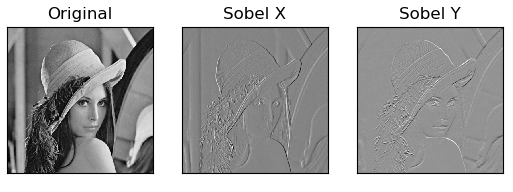
\includegraphics[width=0.8\textwidth]{sobel_lenna.png}
    \caption{Output feature maps after applying $G_x$ and $G_y$, in comparison to the original image (left).}
    \label{fig:sobel_lenna}
\end{figure}

\begin{equation}
    \label{eq:sobel}
    G_x = 
    \begin{pmatrix}
        -1 & 0 & 1 \\
        -2 & 0 & 2 \\
        -1 & 0 & 1 
    \end{pmatrix}
    ,~~~~~~
    G_y = 
    \begin{pmatrix}
        1 & 2 & 1 \\
        0 & 0 & 0 \\
        -1 & -2 & -1
    \end{pmatrix}
\end{equation}

\textit{Convolutional layers} generalize the approach of convolving input feature maps with kernels by using kernels whose parameters are learned through backpropagation.
This means that the kernels do not need to be designed manually, because the network can learn which kernels are needed, depending on the task.
Instead of computing the excitation for each $(i,j)$ position, a \textit{stride} can be defined.
A stride of $x$ indicates that the positions to apply the kernel are incremented by $x$, instead of $1$.

\begin{figure}[htb!]
    \centering
    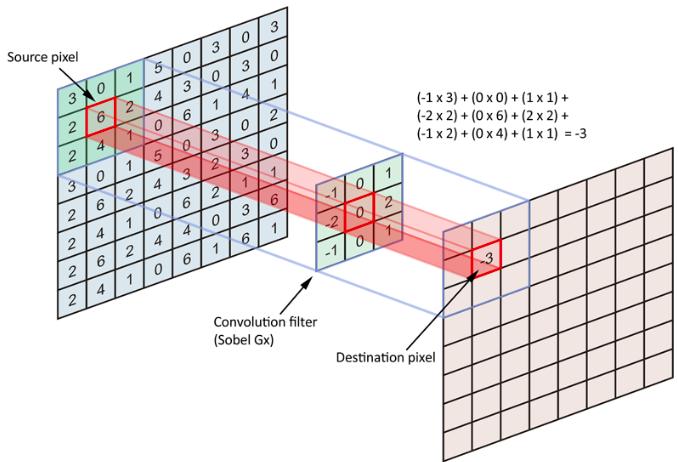
\includegraphics[width=0.8\textwidth]{conv-freecodecamp}
    \caption{Visualisation of using a Sobel filter for detecting vertical edges. Image taken from \cite{dertat_applied_2017}.}
    \label{fig:conv-vis}
\end{figure}

In practice, each convolutional layer consists of multiple kernels.
This results in a output feature map with a depth corresponding to the number of different kernels.
The output feature map can then be processed by another convolutional layer.
A neural network with at least one convolutional layer is also often referred to as a \textbf{Convolutional Neural Network} or a \textbf{CNN}.

% According to \cite{goodfellow_deep_2016}, convolutional layers have three important properties to consider.

% \begin{figure}[htb!]
%     \centering
%     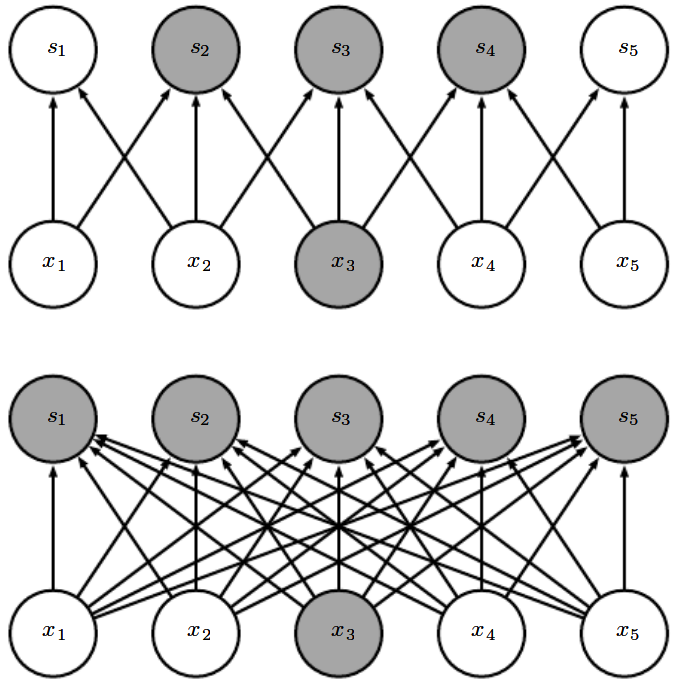
\includegraphics[width=0.8\textwidth]{sparse-connectivity.png}
%     \caption{A visualization of sparse connectivity. Bottom: Connections in a traditional Multi-layer Perceptron. The output of each neuron is connected to the input of all neurons in the successive layer. Top: Connectivity in the case of a three-dimensional kernel. Each neuron is used just three times in order to compute the output of a neuron in the next layer. Image taken from \cite{goodfellow_deep_2016}}
%     \label{fig:sparse-connectivity}
% \end{figure}

% Firstly, a convolution layer utilizes \textbf{sparse connectivity}.
% This means that not all inputs are connected to all neurons in the next layer.
% To illustrate this, consider a one dimensional input vector $\bm{x}$ and a kernel $\bm{k} \in \mathbb{R}^p$.
% By calculating $(\bm{k} * \bm{x})(i)$ for each entry $i$ it becomes clear that each input $\bm{x}_i$ is only used to calculate $p$ output values.
% See \fref{fig:sparse-connectivity} for a visualization.
% Because of this property, the amount of parameters needed reduces drastically.
% Traditionally, $m \cdot n$ parameters would be needed to calculate all output values for $m$ inputs and $n$ neurons.
% Using convolutions, this reduces to $m \cdot p$.

% Secondly, \textbf{parameter sharing} is another important property of convolutional layers.
% Convolutions do not learn one weight per input but a fixed amount of weights defined by the kernel size.
% Because there are only $p^2$ parameters to learn (assuming a two dimensional kernel) as opposed to $m \cdot n$ this further reduces the number of needed parameters.

% Thirdly, convolution layer are \textbf{equivariant to translation}.
% This means that changes in the input result in the same change in the output.
% More specifically, translating the input and then calculating the convolution results in the same output as calculating the convolution first and then applying translation.
% This is useful when considering that a kernel can easily learn to detect edges in the input image.
% Without this property, it would not be guaranteed that the edge detector produces the same output no matter where in the image an edge is occurring.

% padding
Since the kernel is centered at each coordinate $(i,j)$ of the input feature map, a decision has to be made when not all input values are present, e.g., at the edges of an input image.
Generally, there are two approaches used in the literature.
First, $(i,j)$ positions where not all input feature map values are available can be ignored, resulting in a output feature map with smaller spatial dimensions since the convolution was not computed for every $(i,j)$ position.
Second, the missing values can be substituted.
This is referred to as \textbf{padding}.
Common padding approaches are to fill the missing values with $0$ or duplicating with the nearest input feature map values.

\subsubsection{Pooling Layer}
Another important layer type when using Convolutional Neural Networks is the \textit{pooling layer}.
Pooling layers are used to reduce the size of the activation map and introduce invariance to small translations when applied to the spatial dimensions \cite{goodfellow_deep_2016}.
There are different types of pooling layer, however the most popular is the \textbf{Max-pooling} layer where, for each $n \times n$ pixel block, the maximum value is used as the output.
Consider the output feature map of the previously discussed Sobel filter, where high values indicate the presence of a horizontal or vertical edge, depending on the kernel.
In a similar sliding-window approach to the convolutional layer, the Max-pooling layer computes the maximum values for $n \times m$ blocks at each pixel position.
Additionally, a stride $s$ can be defined as well and, in practice, the stride is often set to $s=n$.
This results in a reduction of the spatial dimension of the feature map by a factor $n$ in both dimensions.
Also, invariance to small translations is introduced because the maximum value is propagated, regardless of where in the $n \times n$ window it occured. 
See \fref{fig:pooling-tds} for a visualization.

\begin{figure}[htb!]
    \centering
    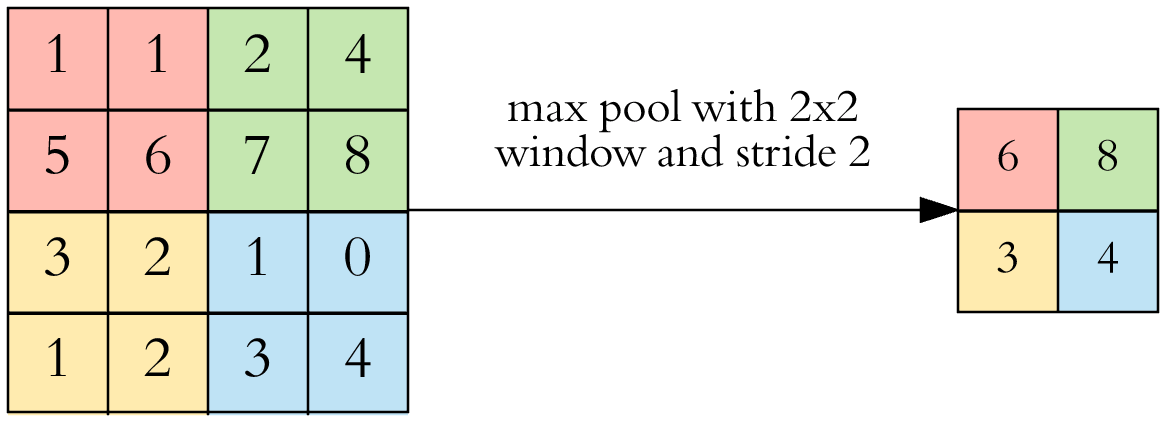
\includegraphics[width=0.65\textwidth]{pooling-tds.png}
    \caption{Example of a $2 \times 2$ Max-pooling operation with a stride of $2$. Image taken from \cite{cornelisse_intuitive_2018}.}
    \label{fig:pooling-tds}
\end{figure}

% Using a pooling layer, the representation becomes invariant to small translations.
% This means that small translations in an input image do not change the output of the pooling layer.
% Pooling layers are useful if it is more important whether or not some feature is present in the image as opposed to finding the exact location.
% For the task of image classification, for example, knowing that the image contains a face is more useful than to know the exact location of the face.

% \begin{figure}[htb!]
%     \centering
%     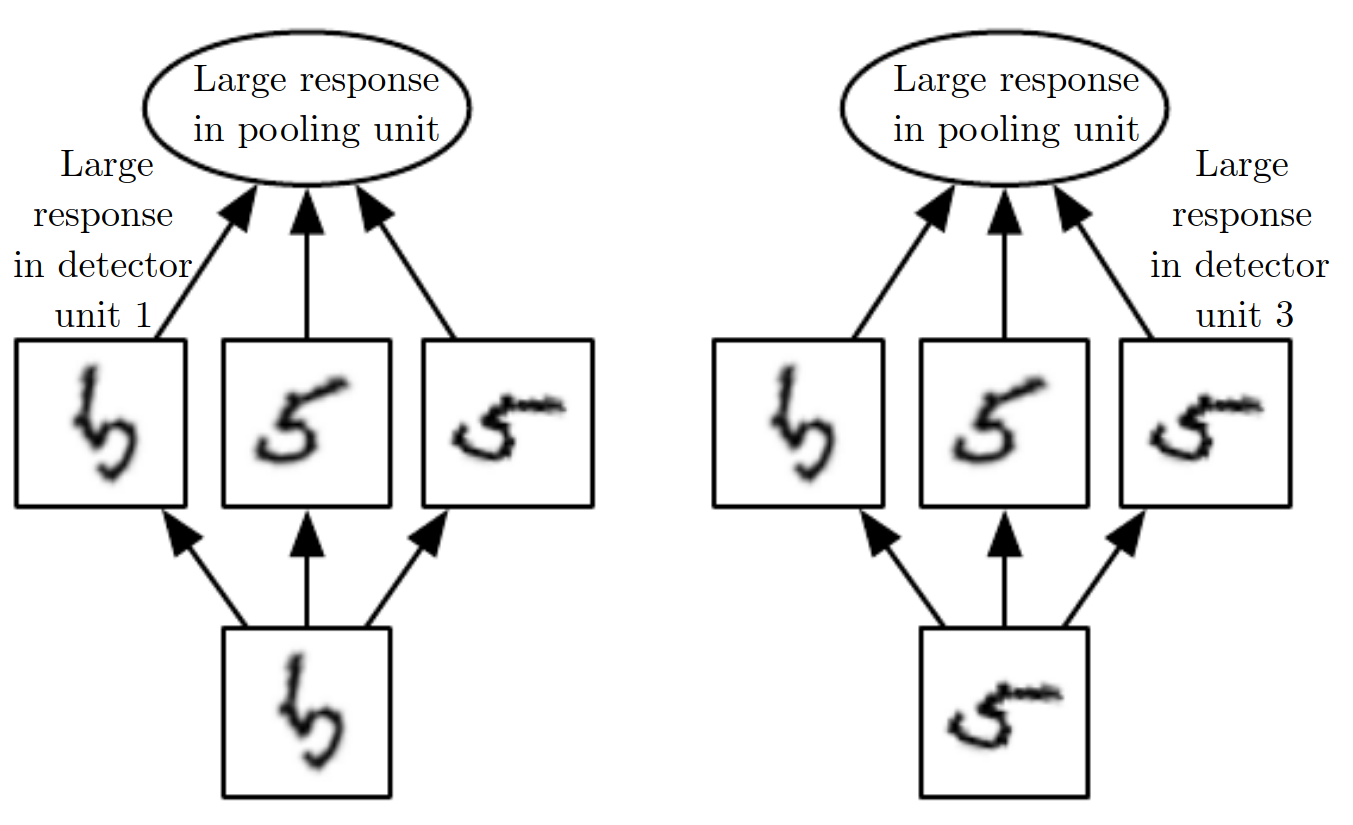
\includegraphics[width=0.8\textwidth]{pooling-goodfellow.png}
%     \caption{Illustration of a Max-pooling layer learning invariance towards rotation. By comparing the input against multiple differently rotated versions and just propagating the highest activation no matter which of the filters ultimately detected the number. Image taken from \cite{goodfellow_deep_2016}.}
%     \label{fig:pooling-goodfellow}
% \end{figure}

% This aspect of invariance towards translation is just an example, however.
% Using a pooling layer, invariance towards specific characteristics can be learned.
% Consider Fig. \ref{fig:pooling-goodfellow} where, using a pooling layer, invariance towards rotation is learned.

\subsubsection{Fully-Connected Layer}
As discussed previously, in convolutional neural networks, convolution and pooling layers are used to extract visual features from the input.
The features can then be used for classifying or regression.
For this purpose, layers of neurons, as introduced earlier, can be added to a convolutional neural network.
In the context of CNNs, these layers are referred to as \textbf{fully-connected} layers.
An example of a CNN where features are computed and then classified can be seen in \fref{fig:cnn_pipeline}.

\begin{figure}[htb!]
    \centering
    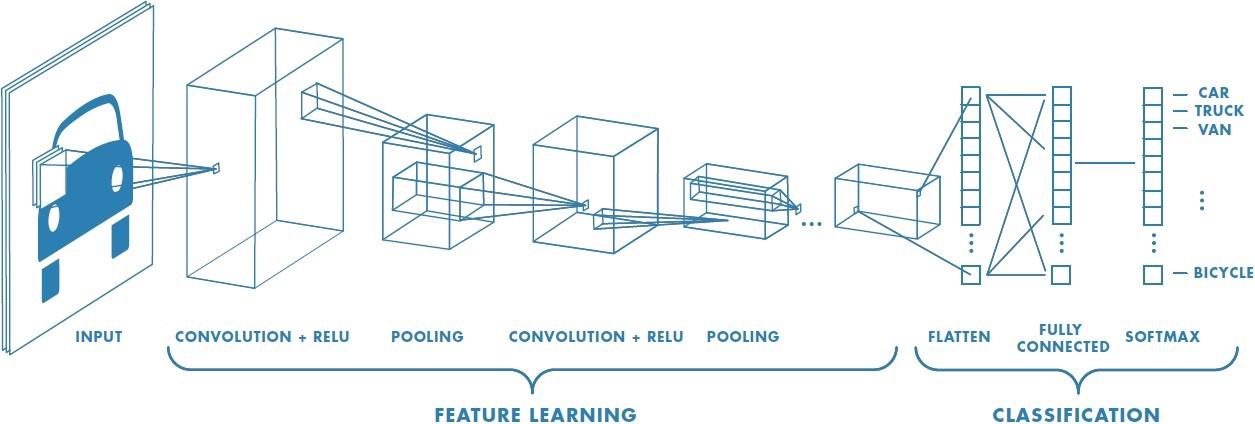
\includegraphics[width=0.8\textwidth]{cnn_pipeline.jpeg}
    \caption{Example of a Convolutional Neural network, consisting of a feature extractor, followed by a fully connected network, which uses the Softmax activation function for classification. Image taken from \cite{saha_comprehensive_2018}.}
    \label{fig:cnn_pipeline}
\end{figure}